\section{Introduction}  \label{sec:Introduction}



\IEEEPARstart{P}{otential}  applications of systems capable of joint sensing and communications include automotive car-to-car communications and cellular sensing \cite{akan2020internet, ma2020joint, ADAS2,Gerstmair1ADAS, ADAS1, Gerstmair2ADAS}. While many different system architectures and waveform designs are possible, a so-called dual-function radar-communication system is assumed in this work that uses the very same transmit signals for both, radar sensing and  communications, simultaneously. Further, it is assumed that the communication receiver and the radar receiver are located at different positions.

A prominent waveform for joint sensing and communication systems is \ac{ofdm}  \cite{Levanon_Multifrequency_complementary, Donnet_Combining_MIMO_Radar, Sturm_A_novel_approach, Garmatyuk_Feasibility_study, Sturm_An_OFDM_System, Sturm_Performance_verification, Sit_Automotive_MIMO_OFDM,Braun_Parametrization, Hakobyan_A_novel_OFDM_MIMO, Hakobyan_Inter_Carrier_Interference, lang2022ofdm}, which is also basis for the investigations in this work.




For many radar sensing applications, detecting the angular positions of objects in the sensor's vicinity is of importance. This is usually achieved by utilizing \ac{dbf} in combination with several transmit (Tx) and receive (Rx) antennas. These so-called \ac{mimo} systems \cite{8443533} employ multiplexing methods for generating orthogonal transmit signals that are separable in the receiver. 
%Multiplexing techniques for the \ac{ofdm} waveform are discussed in \cite{cao2015irci_sar, cao2015irci, xia2015mimo, zhang2014irci, zhang2014ofdm} for radar sensing applications, but without considering simultaneous communications. 
The most popular multiplexing method for the \ac{ofdm} waveform is \ac{esi}  \cite{Sit_Automotive_MIMO_OFDM, sturm2013spectrally}, for which each subcarrier is assigned to only one of the $N_\text{Tx}$ Tx antennas (cf. Fig.~\ref{fig_MIMO_spectral_interleaving} a). Hence, signals radiated by different Tx antennas can be separated in frequency domain. Several extensions of \ac{esi} exist with randomly allocated subcarriers \cite{Knill_Random_Multiplexing}, with non-equidistantly allocated subcarriers \cite{Hakobyan_A_novel_OFDM_MIMO},  and with dynamically allocated subcarriers \cite{Hakobyan_A_novel_OFDM_MIMO_wo_CS}. The latter one is referred to as \ac{dsi}, and it changes the allocation of the subcarriers onto the Tx antennas from \ac{ofdm} symbol to \ac{ofdm} symbol.


%Further multiplexing techniques related to \ac{esi} are discussed in \cite{Hakobyan_A_novel_OFDM_MIMO_wo_CS, Hakobyan_A_novel_OFDM_MIMO, Knill_Random_Multiplexing}. 






%\newcommand\DELTA{0.5}
\begin{figure}[!t]
\centering
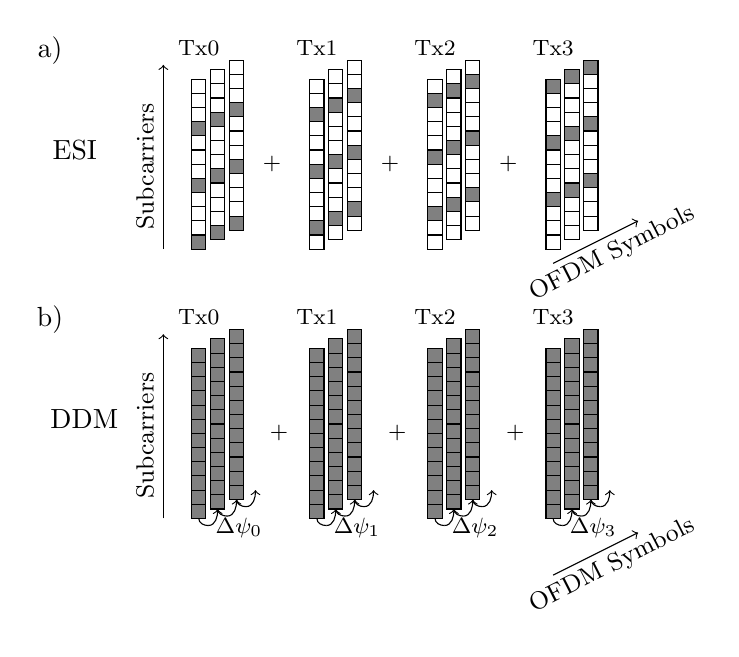
\begin{tikzpicture}[scale=0.6]
\def\d{2.2}%distance between two rows for ESI
\def\dr{2.5}%distance between two rows for RDMult
\def\a{0.3}%width of rectangle
\def\b{3.6}%height of rectangle
\def\hor_dist{5.7}%horizontal distance
\def\dx{0.4}%horizontal distance between symbols
\def\dy{0.2}%vertical distance between symbols

\begin{scope}[shift={(-3*\a,0)}]
%\node[right] at (-1,4.5) {a)};
% Draw axes

	\node at (-10*\a, \b + 2*\a) {a)}; 

	\draw[->] (-2*\a,0)  -- ++(0, \b+\a);
%    \draw [->,thick] (0,3.7) node (yaxis) [above] {}
%        |- (4.2,0) node (xaxis) [right] {};
%    \node[left] at (0,4-\DELTA/2) {\footnotesize $N_\text{c}-1$};    
%    \node[left] at (0,\DELTA/2) {\footnotesize $0$};    
%    \node[below] at (\DELTA/2,0 ) {\footnotesize $0$}; 
%    \node[below, text width=1cm, text centered] at (4 - \DELTA/2,0 ) {\footnotesize $N_\text{sym}-1$}; 
    \node[left, anchor=south, rotate=90] at (-2*\a,1.75) {\small Subcarriers};
%    \node[below] at (2,0) {OFDM symbols};
    

\foreach \inc in {0,...,2}
{	\draw[draw=black, fill=gray] (\inc*\dx,0+\inc*\dy) rectangle ++(\a, \a);
	\draw[draw=black, fill=white] (\inc*\dx,1*\a+\inc*\dy) rectangle ++(\a, \a);
	\draw[draw=black, fill=white] (\inc*\dx,2*\a+\inc*\dy) rectangle ++(\a, \a);
	\draw[draw=black, fill=white] (\inc*\dx,3*\a+\inc*\dy) rectangle ++(\a, \a);
	\draw[draw=black, fill=gray] (\inc*\dx,4*\a+\inc*\dy) rectangle ++(\a, \a);
	\draw[draw=black, fill=white] (\inc*\dx,5*\a+\inc*\dy) rectangle ++(\a, \a);
	\draw[draw=black, fill=white] (\inc*\dx,6*\a+\inc*\dy) rectangle ++(\a, \a);
	\draw[draw=black, fill=white] (\inc*\dx,7*\a+\inc*\dy) rectangle ++(\a, \a);
	\draw[draw=black, fill=gray] (\inc*\dx,8*\a+\inc*\dy) rectangle ++(\a, \a);
	\draw[draw=black, fill=white] (\inc*\dx,9*\a+\inc*\dy) rectangle ++(\a, \a);
	\draw[draw=black, fill=white] (\inc*\dx,10*\a+\inc*\dy) rectangle ++(\a, \a);
	\draw[draw=black, fill=white] (\inc*\dx,11*\a+\inc*\dy) rectangle ++(\a, \a);}

\node[left, anchor=north, rotate=27] at (5*\a ,10*\a) {\small $\hdots$};
	
	\node at (2*\a + 0.5*\d,0.5*\b) {\footnotesize $+$}; 
	\node[above] at (0.5*\a,\b+1*\a) {\footnotesize Tx0};
	

\foreach \inc in {0,...,2}
{	
  \draw[draw=black, fill=white] (\inc*\dx+\a + \d,0+\inc*\dy) rectangle ++(\a, \a);
	\draw[draw=black, fill=gray] (\inc*\dx+\a + \d,1*\a+\inc*\dy) rectangle ++(\a, \a);
	\draw[draw=black, fill=white] (\inc*\dx+\a + \d,2*\a+\inc*\dy) rectangle ++(\a, \a);
	\draw[draw=black, fill=white] (\inc*\dx+\a + \d,3*\a+\inc*\dy) rectangle ++(\a, \a);
	\draw[draw=black, fill=white] (\inc*\dx+\a + \d,4*\a+\inc*\dy) rectangle ++(\a, \a);
	\draw[draw=black, fill=gray] (\inc*\dx+\a + \d,5*\a+\inc*\dy) rectangle ++(\a, \a);
	\draw[draw=black, fill=white] (\inc*\dx+\a + \d,6*\a+\inc*\dy) rectangle ++(\a, \a);
	\draw[draw=black, fill=white] (\inc*\dx+\a + \d,7*\a+\inc*\dy) rectangle ++(\a, \a);
	\draw[draw=black, fill=white] (\inc*\dx+\a + \d,8*\a+\inc*\dy) rectangle ++(\a, \a);
	\draw[draw=black, fill=gray] (\inc*\dx+\a + \d,9*\a+\inc*\dy) rectangle ++(\a, \a);
	\draw[draw=black, fill=white] (\inc*\dx+\a + \d,10*\a+\inc*\dy) rectangle ++(\a, \a);
	\draw[draw=black, fill=white] (\inc*\dx+\a + \d,11*\a+\inc*\dy) rectangle ++(\a, \a);}
	
	\node[left, anchor=north, rotate=27] at (5*\a +\a + \d,10*\a) {\small $\hdots$};
	
%	\draw[draw=black, fill=gray] (\a + \d,\a) rectangle ++(\a, \a);
%	\draw[draw=black, fill=gray] (\a + \d,5*\a) rectangle ++(\a, \a);	
%	\draw[draw=black, fill=gray] (\a + \d,9*\a) rectangle ++(\a, \a);
	
	\node at (3*\a + 1.5*\d,0.5*\b) {\footnotesize $+$}; 
	\node[above] at (1.5*\a+\d,\b+1*\a) {\footnotesize Tx1};
	
\foreach \inc in {0,...,2}
{	\draw[draw=black, fill=white] (\inc*\dx+2*\a + 2*\d,0+\inc*\dy) rectangle ++(\a, \a);
	\draw[draw=black, fill=white] (\inc*\dx+2*\a + 2*\d,1*\a+\inc*\dy) rectangle ++(\a, \a);
	\draw[draw=black, fill=gray] (\inc*\dx+2*\a + 2*\d,2*\a+\inc*\dy) rectangle ++(\a, \a);
	\draw[draw=black, fill=white] (\inc*\dx+2*\a + 2*\d,3*\a+\inc*\dy) rectangle ++(\a, \a);
	\draw[draw=black, fill=white] (\inc*\dx+2*\a + 2*\d,4*\a+\inc*\dy) rectangle ++(\a, \a);
	\draw[draw=black, fill=white] (\inc*\dx+2*\a + 2*\d,5*\a+\inc*\dy) rectangle ++(\a, \a);
	\draw[draw=black, fill=gray] (\inc*\dx+2*\a + 2*\d,6*\a+\inc*\dy) rectangle ++(\a, \a);
	\draw[draw=black, fill=white] (\inc*\dx+2*\a + 2*\d,7*\a+\inc*\dy) rectangle ++(\a, \a);
	\draw[draw=black, fill=white] (\inc*\dx+2*\a + 2*\d,8*\a+\inc*\dy) rectangle ++(\a, \a);
	\draw[draw=black, fill=white] (\inc*\dx+2*\a + 2*\d,9*\a+\inc*\dy) rectangle ++(\a, \a);
	\draw[draw=black, fill=gray] (\inc*\dx+2*\a + 2*\d,10*\a+\inc*\dy) rectangle ++(\a, \a);
	\draw[draw=black, fill=white] (\inc*\dx+2*\a + 2*\d,11*\a+\inc*\dy) rectangle ++(\a, \a);}
	
	\node[left, anchor=north, rotate=27] at (5*\a + 2*\a + 2*\d,10*\a) {\small $\hdots$};
	
%	\draw[draw=black, fill=gray] (2*\a + 2*\d,2*\a) rectangle ++(\a, \a);
%	\draw[draw=black, fill=gray] (2*\a + 2*\d,6*\a) rectangle ++(\a, \a);	
%	\draw[draw=black, fill=gray] (2*\a + 2*\d,10*\a) rectangle ++(\a, \a);
	
	\node at (4*\a + 2.5*\d,0.5*\b) {\footnotesize $+$}; 
	\node[above] at (2.5*\a+2*\d,\b+1*\a) {\footnotesize Tx2};
	
\foreach \inc in {0,...,2}
{	\draw[draw=black, fill=white] (\inc*\dx+3*\a + 3*\d,0+\inc*\dy) rectangle ++(\a, \a);
	\draw[draw=black, fill=white] (\inc*\dx+3*\a + 3*\d,1*\a+\inc*\dy) rectangle ++(\a, \a);
	\draw[draw=black, fill=white] (\inc*\dx+3*\a + 3*\d,2*\a+\inc*\dy) rectangle ++(\a, \a);
	\draw[draw=black, fill=gray] (\inc*\dx+3*\a + 3*\d,3*\a+\inc*\dy) rectangle ++(\a, \a);
	\draw[draw=black, fill=white] (\inc*\dx+3*\a + 3*\d,4*\a+\inc*\dy) rectangle ++(\a, \a);
	\draw[draw=black, fill=white] (\inc*\dx+3*\a + 3*\d,5*\a+\inc*\dy) rectangle ++(\a, \a);
	\draw[draw=black, fill=white] (\inc*\dx+3*\a + 3*\d,6*\a+\inc*\dy) rectangle ++(\a, \a);
	\draw[draw=black, fill=gray] (\inc*\dx+3*\a + 3*\d,7*\a+\inc*\dy) rectangle ++(\a, \a);
	\draw[draw=black, fill=white] (\inc*\dx+3*\a + 3*\d,8*\a+\inc*\dy) rectangle ++(\a, \a);
	\draw[draw=black, fill=white] (\inc*\dx+3*\a + 3*\d,9*\a+\inc*\dy) rectangle ++(\a, \a);
	\draw[draw=black, fill=white] (\inc*\dx+3*\a + 3*\d,10*\a+\inc*\dy) rectangle ++(\a, \a);
	\draw[draw=black, fill=gray] (\inc*\dx+3*\a + 3*\d,11*\a+\inc*\dy) rectangle ++(\a, \a);}
	
	\node[left, anchor=north, rotate=27] at (5*\a+3*\a + 3*\d ,10*\a) {\small $\hdots$};
	
	\draw[->] (\a/2+3*\a + 3*\d,-\a)  -- ++(6*\a, 3*\a);
	\node[left, anchor=north, rotate=27] at (7*\a + 3*\d,1*\a) {\small OFDM Symbols};
	
	\node[above] at (3.5*\a+3*\d,\b+1*\a) {\footnotesize Tx3};
	%\node[above] at (2*\a+1.5*\d,\b+3*\a) {ESI};
	\node[left] at (-6*\a,0.5*\b+1*\a) {ESI};
\end{scope}

  
  \begin{scope}[shift={(-3*\a,-\hor_dist)}]

	\node at (-10*\a, \b + 2*\a) {b)}; 
	\node[left] at (-4.5*\a,0.5*\b+1*\a) {DDM};

	\draw[->] (-2*\a,0)  -- ++(0, \b+\a);
    \node[left, anchor=south, rotate=90] at (-2*\a,1.75) {\small Subcarriers};
    
\foreach \inc in {0,...,2}
{	\draw[draw=black, fill=gray] (\inc*\dx+0,0+\inc*\dy) rectangle ++(\a, \a);
	\draw[draw=black, fill=gray] (\inc*\dx+0,1*\a+\inc*\dy) rectangle ++(\a, \a);
	\draw[draw=black, fill=gray] (\inc*\dx+0,2*\a+\inc*\dy) rectangle ++(\a, \a);
	\draw[draw=black, fill=gray] (\inc*\dx+0,3*\a+\inc*\dy) rectangle ++(\a, \a);
	\draw[draw=black, fill=gray] (\inc*\dx+0,4*\a+\inc*\dy) rectangle ++(\a, \a);
	\draw[draw=black, fill=gray] (\inc*\dx+0,5*\a+\inc*\dy) rectangle ++(\a, \a);
	\draw[draw=black, fill=gray] (\inc*\dx+0,6*\a+\inc*\dy) rectangle ++(\a, \a);
	\draw[draw=black, fill=gray] (\inc*\dx+0,7*\a+\inc*\dy) rectangle ++(\a, \a);
	\draw[draw=black, fill=gray] (\inc*\dx+0,8*\a+\inc*\dy) rectangle ++(\a, \a);
	\draw[draw=black, fill=gray] (\inc*\dx+0,9*\a+\inc*\dy) rectangle ++(\a, \a);
	\draw[draw=black, fill=gray] (\inc*\dx+0,10*\a+\inc*\dy) rectangle ++(\a, \a);
	\draw[draw=black, fill=gray] (\inc*\dx+0,11*\a+\inc*\dy) rectangle ++(\a, \a);}
	
		\node[left, anchor=north, rotate=27] at (5*\a ,10*\a) {\small $\hdots$};
		
		
	
	\draw [-] (0.5*\a, 0) to [out=270,in=180] (0.5*\a+0.5*\dx, -0.5*\a);
	\draw [->] (0.5*\a+0.5*\dx, -0.5*\a) to [out=0,in=270] (0.5*\a+\dx, 0+\dy);
	\draw [-] (0.5*\a+\dx, 0+\dy) to [out=270,in=180] (0.5*\a+0.5*\dx+\dx, -0.5*\a+\dy);
	\draw [->] (0.5*\a+0.5*\dx+\dx, -0.5*\a+\dy) to [out=0,in=270] (0.5*\a+\dx+\dx, 0+\dy+\dy);
	\draw [-] (0.5*\a+2*\dx, 0+2*\dy) to [out=270,in=180] (0.5*\a+0.5*\dx+2*\dx, -0.5*\a+2*\dy);
	\draw [->] (0.5*\a+0.5*\dx+2*\dx, -0.5*\a+2*\dy) to [out=0,in=270] (0.5*\a+\dx+2*\dx, 0+\dy+2*\dy);
	
	\node[right] at (1*\a ,-0.7*\a) {\footnotesize $\Delta \psi_0$}; 
	
	\node at (2*\a + 0.5*\dr,0.5*\b) {\footnotesize $+$}; 
	\node[above] at (0.5*\a,\b+1*\a) {\footnotesize Tx0};
	

\end{scope}

\begin{scope}[shift={(\dr-3*\a,-\hor_dist)}]
    
\foreach \inc in {0,...,2}
{	\draw[draw=black, fill=gray] (\inc*\dx+0,0+\inc*\dy) rectangle ++(\a, \a);
	\draw[draw=black, fill=gray] (\inc*\dx+0,1*\a+\inc*\dy) rectangle ++(\a, \a);
	\draw[draw=black, fill=gray] (\inc*\dx+0,2*\a+\inc*\dy) rectangle ++(\a, \a);
	\draw[draw=black, fill=gray] (\inc*\dx+0,3*\a+\inc*\dy) rectangle ++(\a, \a);
	\draw[draw=black, fill=gray] (\inc*\dx+0,4*\a+\inc*\dy) rectangle ++(\a, \a);
	\draw[draw=black, fill=gray] (\inc*\dx+0,5*\a+\inc*\dy) rectangle ++(\a, \a);
	\draw[draw=black, fill=gray] (\inc*\dx+0,6*\a+\inc*\dy) rectangle ++(\a, \a);
	\draw[draw=black, fill=gray] (\inc*\dx+0,7*\a+\inc*\dy) rectangle ++(\a, \a);
	\draw[draw=black, fill=gray] (\inc*\dx+0,8*\a+\inc*\dy) rectangle ++(\a, \a);
	\draw[draw=black, fill=gray] (\inc*\dx+0,9*\a+\inc*\dy) rectangle ++(\a, \a);
	\draw[draw=black, fill=gray] (\inc*\dx+0,10*\a+\inc*\dy) rectangle ++(\a, \a);
	\draw[draw=black, fill=gray] (\inc*\dx+0,11*\a+\inc*\dy) rectangle ++(\a, \a);}
	
		\node[left, anchor=north, rotate=27] at (5*\a ,10*\a) {\small $\hdots$};
		
		
	\draw [-] (0.5*\a, 0) to [out=270,in=180] (0.5*\a+0.5*\dx, -0.5*\a);
	\draw [->] (0.5*\a+0.5*\dx, -0.5*\a) to [out=0,in=270] (0.5*\a+\dx, 0+\dy);
	\draw [-] (0.5*\a+\dx, 0+\dy) to [out=270,in=180] (0.5*\a+0.5*\dx+\dx, -0.5*\a+\dy);
	\draw [->] (0.5*\a+0.5*\dx+\dx, -0.5*\a+\dy) to [out=0,in=270] (0.5*\a+\dx+\dx, 0+\dy+\dy);
	\draw [-] (0.5*\a+2*\dx, 0+2*\dy) to [out=270,in=180] (0.5*\a+0.5*\dx+2*\dx, -0.5*\a+2*\dy);
	\draw [->] (0.5*\a+0.5*\dx+2*\dx, -0.5*\a+2*\dy) to [out=0,in=270] (0.5*\a+\dx+2*\dx, 0+\dy+2*\dy);
	
	\node[right] at (1*\a ,-0.7*\a) {\footnotesize $\Delta \psi_1$}; 
	
	\node at (2*\a + 0.5*\dr,0.5*\b) {\footnotesize $+$}; 
	\node[above] at (0.5*\a,\b+1*\a) {\footnotesize Tx1};
	

\end{scope}

\begin{scope}[shift={(2*\dr-3*\a,-\hor_dist)}]
    
\foreach \inc in {0,...,2}
{	\draw[draw=black, fill=gray] (\inc*\dx+0,0+\inc*\dy) rectangle ++(\a, \a);
	\draw[draw=black, fill=gray] (\inc*\dx+0,1*\a+\inc*\dy) rectangle ++(\a, \a);
	\draw[draw=black, fill=gray] (\inc*\dx+0,2*\a+\inc*\dy) rectangle ++(\a, \a);
	\draw[draw=black, fill=gray] (\inc*\dx+0,3*\a+\inc*\dy) rectangle ++(\a, \a);
	\draw[draw=black, fill=gray] (\inc*\dx+0,4*\a+\inc*\dy) rectangle ++(\a, \a);
	\draw[draw=black, fill=gray] (\inc*\dx+0,5*\a+\inc*\dy) rectangle ++(\a, \a);
	\draw[draw=black, fill=gray] (\inc*\dx+0,6*\a+\inc*\dy) rectangle ++(\a, \a);
	\draw[draw=black, fill=gray] (\inc*\dx+0,7*\a+\inc*\dy) rectangle ++(\a, \a);
	\draw[draw=black, fill=gray] (\inc*\dx+0,8*\a+\inc*\dy) rectangle ++(\a, \a);
	\draw[draw=black, fill=gray] (\inc*\dx+0,9*\a+\inc*\dy) rectangle ++(\a, \a);
	\draw[draw=black, fill=gray] (\inc*\dx+0,10*\a+\inc*\dy) rectangle ++(\a, \a);
	\draw[draw=black, fill=gray] (\inc*\dx+0,11*\a+\inc*\dy) rectangle ++(\a, \a);}
	
		\node[left, anchor=north, rotate=27] at (5*\a ,10*\a) {\small $\hdots$};
	
	\draw [-] (0.5*\a, 0) to [out=270,in=180] (0.5*\a+0.5*\dx, -0.5*\a);
	\draw [->] (0.5*\a+0.5*\dx, -0.5*\a) to [out=0,in=270] (0.5*\a+\dx, 0+\dy);
	\draw [-] (0.5*\a+\dx, 0+\dy) to [out=270,in=180] (0.5*\a+0.5*\dx+\dx, -0.5*\a+\dy);
	\draw [->] (0.5*\a+0.5*\dx+\dx, -0.5*\a+\dy) to [out=0,in=270] (0.5*\a+\dx+\dx, 0+\dy+\dy);
	\draw [-] (0.5*\a+2*\dx, 0+2*\dy) to [out=270,in=180] (0.5*\a+0.5*\dx+2*\dx, -0.5*\a+2*\dy);
	\draw [->] (0.5*\a+0.5*\dx+2*\dx, -0.5*\a+2*\dy) to [out=0,in=270] (0.5*\a+\dx+2*\dx, 0+\dy+2*\dy);
	
	\node[right] at (1*\a ,-0.7*\a) {\footnotesize $\Delta \psi_2$}; 
	
	\node at (2*\a + 0.5*\dr,0.5*\b) {\footnotesize $+$}; 
	\node[above] at (0.5*\a,\b+1*\a) {\footnotesize Tx2};
	

\end{scope}
\begin{scope}[shift={(3*\dr-3*\a,-\hor_dist)}]
    
\foreach \inc in {0,...,2}
{	\draw[draw=black, fill=gray] (\inc*\dx+0,0+\inc*\dy) rectangle ++(\a, \a);
	\draw[draw=black, fill=gray] (\inc*\dx+0,1*\a+\inc*\dy) rectangle ++(\a, \a);
	\draw[draw=black, fill=gray] (\inc*\dx+0,2*\a+\inc*\dy) rectangle ++(\a, \a);
	\draw[draw=black, fill=gray] (\inc*\dx+0,3*\a+\inc*\dy) rectangle ++(\a, \a);
	\draw[draw=black, fill=gray] (\inc*\dx+0,4*\a+\inc*\dy) rectangle ++(\a, \a);
	\draw[draw=black, fill=gray] (\inc*\dx+0,5*\a+\inc*\dy) rectangle ++(\a, \a);
	\draw[draw=black, fill=gray] (\inc*\dx+0,6*\a+\inc*\dy) rectangle ++(\a, \a);
	\draw[draw=black, fill=gray] (\inc*\dx+0,7*\a+\inc*\dy) rectangle ++(\a, \a);
	\draw[draw=black, fill=gray] (\inc*\dx+0,8*\a+\inc*\dy) rectangle ++(\a, \a);
	\draw[draw=black, fill=gray] (\inc*\dx+0,9*\a+\inc*\dy) rectangle ++(\a, \a);
	\draw[draw=black, fill=gray] (\inc*\dx+0,10*\a+\inc*\dy) rectangle ++(\a, \a);
	\draw[draw=black, fill=gray] (\inc*\dx+0,11*\a+\inc*\dy) rectangle ++(\a, \a);}
	

		\draw [-] (0.5*\a, 0) to [out=270,in=180] (0.5*\a+0.5*\dx, -0.5*\a);
	\draw [->] (0.5*\a+0.5*\dx, -0.5*\a) to [out=0,in=270] (0.5*\a+\dx, 0+\dy);
	\draw [-] (0.5*\a+\dx, 0+\dy) to [out=270,in=180] (0.5*\a+0.5*\dx+\dx, -0.5*\a+\dy);
	\draw [->] (0.5*\a+0.5*\dx+\dx, -0.5*\a+\dy) to [out=0,in=270] (0.5*\a+\dx+\dx, 0+\dy+\dy);
	\draw [-] (0.5*\a+2*\dx, 0+2*\dy) to [out=270,in=180] (0.5*\a+0.5*\dx+2*\dx, -0.5*\a+2*\dy);
	\draw [->] (0.5*\a+0.5*\dx+2*\dx, -0.5*\a+2*\dy) to [out=0,in=270] (0.5*\a+\dx+2*\dx, 0+\dy+2*\dy);
	
	\node[right] at (1*\a ,-0.7*\a) {\footnotesize $\Delta \psi_3$}; 
	
	
	\node[left, anchor=north, rotate=27] at (5*\a ,10*\a) {\small $\hdots$};
	
	\node[above] at (0.5*\a,\b+1*\a) {\footnotesize Tx3};
	
		\draw[->] (\a/2+3*\a + 3*\d-3*\dr,-4*\a)  -- ++(6*\a, 3*\a);
	\node[left, anchor=north, rotate=27] at (7*\a + 3*\d-3*\dr,-2*\a) {\small OFDM Symbols};

\end{scope}



\end{tikzpicture}
 \caption{a) Schematic visualization of the subcarrier allocation for ESI for the special case of 4 Tx antennas. Only every 4th subcarrier is active (gray blocks) for each Tx antenna. b) Sketch of the principle of DDM with unique phase shifts $\Delta \psi_k$ from OFDM symbol to OFDM symbol that shifts the received signals along the velocity axis. $k$ denotes the Tx antenna index. }
\label{fig_MIMO_spectral_interleaving}
\end{figure}





A multiplexing method analyzed in \cite{knill2021coded} is denoted as \ac{accdm}. For this method, the same data are radiated on every Tx antenna and on every subcarrier except for antenna-specific time delays. These time delays, which are implemented via linearly increasing phase rotations along the subcarriers, move the corresponding receive signals along the range axis of the \ac{rvm} such that $N_\text{Tx}$ peaks appear along the range axis for each real object.
%, whereas $N_\text{Tx}-1$ of them are ambiguous peaks. These ambiguous peaks may be identified by choosing irregular time delays for the $N_\text{Tx}$ transmitters \cite{knill2021coded}. 


Another multiplexing method analyzed in \cite{knill2021coded} is denoted as \ac{mrscdm}, which applies orthogonal Hadamard codes onto the \ac{ofdm} symbols transmitted by different Tx antennas. In the receiver, $N_\text{Tx}$ \acp{rvm} are evaluated separately, one for each Tx antenna. In every \ac{rvm} there appears one main peak and $N_\text{Tx}-1$ spurs along the velocity axis for each real object such that the maximum unambiguous velocity is reduced by a factor of $N_\text{Tx}$.

A \ac{dft}-coded multiplexing method investigated in \cite{suh2021time} applies a \ac{dft} matrix as precoding matrix onto the transmit signals that shifts the corresponding receive signals either along the range axis, the velocity axis, or both of them. 

The multiplexing method analyzed in \cite{Lang_RDM_JP} is referred to as \ac{rdm}, and it applies a phase shift from subcarrier to subcarrier to shift the signal components of the \ac{rvm} along the range axis. The transmit signals generated by \ac{rdm} coincide with that generated by \ac{accdm} \cite{knill2021coded} and the \ac{dft}-coded multiplexing method \cite{suh2021time} for special parametrization \cite{Lang_RDM_JP}. 




%Several multiplexing techniques similar to \ac{esi} exist in published literature. In \cite{Hakobyan_A_novel_OFDM_MIMO_wo_CS}, dynamic allocation of the subcarriers is discussed, which unfortunately increases the noise floor. \cite{Hakobyan_A_novel_OFDM_MIMO} contains a multiplexing technique with non-equidistant allocated subcarriers, while random time-dependent allocation is analyzed in \cite{Knill_Random_Multiplexing}. Both techniques employ computationally expensive \ac{cs} methods to reduce negative side-effects. 

%\begin{table}[!t]
%% increase table row spacing, adjust to taste
%\renewcommand{\arraystretch}{1.3}
% %if using array.sty, it might be a good idea to tweak the value of
% %\extrarowheight as needed to properly center the text within the cells
%\caption{Overview of achieved values for $r_\text{max}$ and  $v_\text{max}$ for practical radar applications found in the literature. This table is taken from \cite{Lang_Asilomar_2020}.}
%\label{Tab:Overview_max_vals}
%\centering
%% Some packages, such as MDW tools, offer better commands for making tables
%% than the plain LaTeX2e tabular which is used here.
%\begin{tabular}{|l|r|r|}
%\hline
%Reference & $r_\text{max}$ (m) & $v_\text{max}$ (m/s) \\
%\hline 
%\cite{Hakobyan_Inter_Carrier_Interference} (sim) & $1536$ &  $\pm 95$ \\
%\hline
%\cite{Hakobyan_Inter_Carrier_Interference} (meas) & $16384$ &  $\pm 28$ \\
%\hline
%\cite{Sturm_A_novel_approach} & $1650$ &  - \\
%\hline
%\cite{Braun_Parametrization} & $360$ &  $\pm 221$ \\
%\hline
%\cite{Sit_An_overview} & $1650$ &  $\pm 252$ \\
%\hline
%\cite{Comb_OFDM} & $77$ & $\pm 371$ \\
%\hline
%\end{tabular}
%\end{table}


%The \ac{ofdm} waveform features four key performance measures \cite{Lang_Asilomar_2020} \ac{wrt} a radar application: the maximum unambiguous range $r_\text{max}$, the range resolution $\Delta r$, the maximum unambiguous relative velocity $v_\text{max}$, and the velocity resolution $\Delta v$. These key performance measures shall be chosen to match the demands of modern automotive radar systems. However, due to a shortage of freely selectable design parameters, which is discussed in \cite{Lang_Asilomar_2020}, not every performance measure can be chosen independently. This is the reason why many \ac{ofdm} radar systems in the literature feature by far too large values for $r_\text{max}$ and/or $v_\text{max}$. Tab.~\ref{Tab:Overview_max_vals} shows some examples from the literature. For these radar systems, one can assume that large areas in the \ac{rvm} will be free of objects all the time. 
%This can easily be seen when comparing the values of $v_\text{max}$ in Tab.~\ref{Tab:Overview_max_vals} with the speed of sound, which is around $340\, \text{m/s}$. 
%Similarly, combining the large values for $r_\text{max}$ with the dissipation of the signal power, which is proportional to the distance to the power of 4, shows that practically no signal is received from objects at these distances. 
%One can conclude, that the large values for $r_\text{max}$ and/or $v_\text{max}$ generate areas in the \ac{rvm}, which are free of objects. 

%Possible countermeasures are discussed in \cite{Lang_Asilomar_2020}. There, a decimation step in the receiver signal processing chain is proposed, which allows to drastically reduce the computational burden and the hardware requirements for \ac{ofdm} radar systems with only a minor degradation of the \ac{snr}.




\begin{figure}[!t]
\centering
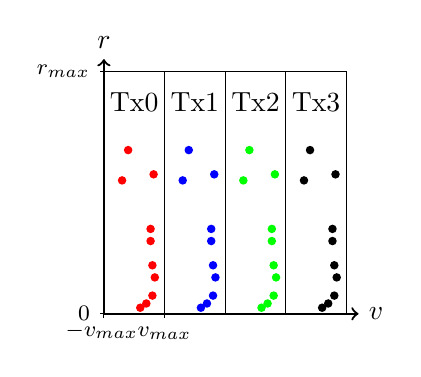
\begin{tikzpicture}[scale=0.77]
% Draw axes
%	\node[above] at (2,4) {SISO};
%
%    \draw [<->,thick] (0,4.2) node (yaxis) [above] {$r$}
%        |- (4.2,0) node (xaxis) [right] {$v$};
%    \draw[draw = black] (0pt,2pt) -- (0pt,-2pt) node[below] {\footnotesize $-v_\text{max}$};
%    \draw[draw = black] (2,2pt) -- (2,-2pt) node[below] {\footnotesize $0$};
%    \draw[draw = black] (4,2pt) -- (4,-2pt) node[below] {\footnotesize $v_\text{max}$};
%    \draw[draw = black] (2pt,0) -- (-2pt,0) node[left] {\footnotesize $0$};
%    \draw[draw = black] (2pt,4) -- (-2pt,4) node[left] {\footnotesize $r_\text{max}$};
%% Draw rectangles
%    \draw[draw=black] (0,0) rectangle ++(4,4);
%% Draw Objects
%    \fill[red] (1.8,2.2) circle (2pt);
%    \fill[red] (1.9,2.7) circle (2pt);
%    \fill[red] (2.1,0.1) circle (2pt);
%    \fill[red] (2.2,0.17) circle (2pt);
%    \fill[red] (2.3,0.3) circle (2pt);
%    \fill[red] (2.34,0.6) circle (2pt);
%    \fill[red] (2.3,0.8) circle (2pt);
%    \fill[red] (2.27,1.2) circle (2pt);
%    \fill[red] (2.27,1.4) circle (2pt);
%    \fill[red] (2.32,2.3) circle (2pt);
%    %
%\node[ align = center, rotate = 85] at (0.75,2) {\small Usually free of objects};
%\node[ align = center, rotate = 85] at (3.25,2) {\small Usually free of objects};
%\draw[draw = none, fill=gray, fill opacity=0.2, draw opacity=0] (0,0) rectangle ++(1.5,4);
%\draw[draw = none, fill=gray, fill opacity=0.2, draw opacity=0] (2.5,0) rectangle ++(1.5,4);
    % 
    \begin{scope}[shift={(5.3,0)}]
   % \node[above] at (2,4) {DDM};
    % Draw axes
    \draw [<->,thick] (0,4.2) node (yaxis) [above] {$r$}
        |- (4.2,0) node (xaxis) [right] {$v$};
%    \draw[draw = black] (0pt,2pt) -- (0pt,-2pt) node[below] {\footnotesize $-v_\text{max}$};
%    \draw[draw = black] (2,2pt) -- (2,-2pt) node[below] {\footnotesize $0$};
%    \draw[draw = black] (4,2pt) -- (4,-2pt) node[below] {\footnotesize $v_\text{max}$};
    \draw[draw = black] (2pt,0) -- (-2pt,0) node[left] {\footnotesize $0$};
    \draw[draw = black] (2pt,4) -- (-2pt,4) node[left] {\footnotesize $r_\text{max}$};

% Draw rectangles
    \draw[draw=black] (0,0) rectangle ++(1,4);
    \draw[draw=black] (1,0) rectangle ++(1,4);
    \draw[draw=black] (2,0) rectangle ++(1,4);
    \draw[draw=black] (3,0) rectangle ++(1,4);
% Draw Tx indication
    \node[align = center] at (0.5,3.5) {Tx0};
    \node[align = center] at (1.5,3.5) {Tx1};
    \node[align = center] at (2.5,3.5) {Tx2};
    \node[align = center] at (3.5,3.5) {Tx3};
% Draw Objects
	\fill[red] (1.8-1.5,2.2) circle (2pt);
    \fill[red] (1.9-1.5,2.7) circle (2pt);
    \fill[red] (2.1-1.5,0.1) circle (2pt);
    \fill[red] (2.2-1.5,0.17) circle (2pt);
    \fill[red] (2.3-1.5,0.3) circle (2pt);
    \fill[red] (2.34-1.5,0.6) circle (2pt);
    \fill[red] (2.3-1.5,0.8) circle (2pt);
    \fill[red] (2.27-1.5,1.2) circle (2pt);
    \fill[red] (2.27-1.5,1.4) circle (2pt);
    \fill[red] (2.32-1.5,2.3) circle (2pt);
    
    \fill[blue] (1.8-0.5,2.2) circle (2pt);
    \fill[blue] (1.9-0.5,2.7) circle (2pt);
    \fill[blue] (2.1-0.5,0.1) circle (2pt);
    \fill[blue] (2.2-0.5,0.17) circle (2pt);
    \fill[blue] (2.3-0.5,0.3) circle (2pt);
    \fill[blue] (2.34-0.5,0.6) circle (2pt);
    \fill[blue] (2.3-0.5,0.8) circle (2pt);
    \fill[blue] (2.27-0.5,1.2) circle (2pt);
    \fill[blue] (2.27-0.5,1.4) circle (2pt);
    \fill[blue] (2.32-0.5,2.3) circle (2pt);
    
	\fill[green] (1.8+0.5,2.2) circle (2pt);
    \fill[green] (1.9+0.5,2.7) circle (2pt);
    \fill[green] (2.1+0.5,0.1) circle (2pt);
    \fill[green] (2.2+0.5,0.17) circle (2pt);
    \fill[green] (2.3+0.5,0.3) circle (2pt);
    \fill[green] (2.34+0.5,0.6) circle (2pt);
    \fill[green] (2.3+0.5,0.8) circle (2pt);
    \fill[green] (2.27+0.5,1.2) circle (2pt);
    \fill[green] (2.27+0.5,1.4) circle (2pt);
    \fill[green] (2.32+0.5,2.3) circle (2pt);

    \fill[black] (1.8+1.5,2.2) circle (2pt);
    \fill[black] (1.9+1.5,2.7) circle (2pt);
    \fill[black] (2.1+1.5,0.1) circle (2pt);
    \fill[black] (2.2+1.5,0.17) circle (2pt);
    \fill[black] (2.3+1.5,0.3) circle (2pt);
    \fill[black] (2.34+1.5,0.6) circle (2pt);
    \fill[black] (2.3+1.5,0.8) circle (2pt);
    \fill[black] (2.27+1.5,1.2) circle (2pt);
    \fill[black] (2.27+1.5,1.4) circle (2pt);
    \fill[black] (2.32+1.5,2.3) circle (2pt);
    
    \draw[draw = black] (1,2pt) -- (1,-2pt);% node[below] {\footnotesize $v_\text{max}$};
    \draw[draw = black] (0,2pt) -- (0,-2pt);% node[below] {\footnotesize $-v_\text{max}$};
    
    \node at (-1pt,-8pt) {\footnotesize $-v_\text{max}$};
	\node at (1,-9pt) {\footnotesize $v_\text{max}$};
	
	
  \end{scope}
\end{tikzpicture}
\caption{ Sketch of an RDM for DDM with $N_\text{Tx}=4$ transmit antennas. Every real object results in $N_\text{Tx}$ peaks in the RDM, each one associated with one Tx antenna. }
\label{fig_DDM_DDM}
\end{figure}

%\input{./fig/Fig_DDM_MIMO_range_Doppler_map_R1}


In this work, we analyze a multiplexing method referred to as \ac{ddm}. \ac{ddm} shares some similarities with the \ac{dft}-coded multiplexing method \cite{suh2021time}, with \ac{mrscdm} \cite{knill2021coded}, and with \ac{rdm} \cite{Lang_RDM_JP}, however, there exist distinct differences in some details that will be discussed later. 
\ac{ddm} modifies the transmit signal for each Tx antenna such that the received signal components are shifted along the velocity axis. A proper modification to achieve this is a Tx antenna specific phase shift from \ac{ofdm} symbol to \ac{ofdm} symbol as indicated in  Fig.~\ref{fig_MIMO_spectral_interleaving} b). This phase shift is referred to as $\Delta \psi_k$, with the Tx antenna index $k=0,1, \hdots, N_\text{Tx}-1$. 
%Applyin of the transmit signals requires only minimal computational complexity as will be shown. 
A schematic \ac{rvm} for a \ac{mimo} \ac{ofdm} radar system utilizing \ac{ddm} is sketched in Fig.~\ref{fig_DDM_DDM} for $N_\text{Tx} = 4$ Tx antennas. This figure shows a possible alignment of the Tx antennas and their corresponding signal components within the \ac{rvm}. 
%A separation of the signal components in the velocity domain allows utilizing all subcarriers for every Tx antenna in every \ac{ofdm} symbol. 
For radar sensing, the performance in terms of the \ac{snr} in the \ac{rvm} of a \ac{mimo} \ac{ofdm} radar system utilizing \ac{ddm} is
approximately equal to a \ac{mimo} \ac{ofdm} radar system employing \ac{esi}, which is analyzed in this work. 



%The biggest advantage of \ac{ddm} is a higher processing gain compared to \ac{esi}. This higher processing gain is achieved by activating all subcarriers for every Tx antenna in every \ac{ofdm} symbol. 

%The effects of \ac{ddm} on the communication task are investigated in this work. 



%approach presented in \cite{suh2021time}, with \ac{mrscdm} \cite{knill2021coded}, and with \ac{rdm} \cite{Lang_RDM_JP}
\ac{ddm} shares some similarities with the \ac{dft}-coded multiplexing method \cite{suh2021time}, which utilizes a \ac{dft} precoding matrix applied on the subcarriers and/or on the \ac{ofdm} symbols to shift the signal components radiated by different Tx antennas either along the range axis, the velocity axis, or both of them. This \ac{dft} precoding matrix, when applied onto full \ac{ofdm} symbols, corresponds to a phase shift from \ac{ofdm} symbol to \ac{ofdm} symbol as done for \ac{ddm}. However, the design rule for choosing the phase shift utilized in this work differs from the one employed in \cite{suh2021time} (cf. Sec.~\ref{sec.Choice_of_phi}). Moreover, no analysis of the implications of the phase shift on the communication task was carried out if \cite{suh2021time}.

 \ac{ddm} also shares some similarities with \ac{mrscdm} \cite{knill2021coded} by means of shifting signal components from different Tx antennas along the velocity axis. However, for \ac{mrscdm}, each Tx antenna repeatedly transmits the same \ac{ofdm} symbol during a whole frame of $N_\text{sym}$ \ac{ofdm} symbols, preventing efficient communications. In contrast to that, \ac{ddm} allows for efficient communications as will be demonstrated in this work. Moreover, the orthogonal Hadamard codes applied on the transmit \ac{ofdm} symbols for \ac{mrscdm} in general differ from the phase shift utilized in \ac{ddm} (cf. Sec.~\ref{sec.Choice_of_phi}).


%A multiplexing technique similar to the proposed one already exists for \ac{fmcw} radar systems  \cite{ADAS1, sun2014analysis} and for pulse-Doppler radar systems \cite{FMCW_RDM3, FMCW_RDM2, cao2018slow, mecca2008beamspace}, where it is often referred to as \textit{Doppler-division multiple access}. However, to the best knowledge of the authors, \ac{ddm} has not been analyzed for \ac{ofdm} joint radar and communication systems in the literature.  

The multiplexing methods \ac{rdm} and \ac{ddm} share some similarities, too. Both methods modify the transmit signals such that the corresponding received signals appear in different areas within the \ac{rvm}. However, they have the following differences (with a detailed explanation later in this work)
\begin{itemize}
\item \ac{rdm} applies a phase shift from subcarrier to subcarrier, \ac{ddm} applies a phase shift from \ac{ofdm} symbol to \ac{ofdm} symbol.
\item For \ac{rdm}, the effective communication channel shows a repetitive pattern with constructive/destructive interferences along the subcarriers, while the effective communication channel for \ac{ddm} shows a repetitive pattern with constructive/destructive interferences along the \ac{ofdm} symbols.
\item Both approaches add additional data redundancy to surpass the issue of the mentioned  interferences. This is done by transmitting the same information over several subcarriers for \ac{rdm}, and by transmitting the same information over several \ac{ofdm} symbols for \ac{ddm}. 
\item Naturally, these different approaches of adding additional redundancy require different methods for synchronization, channel estimation, and data estimation.
\end{itemize}


As already mentioned, this work considers so-called dual-function radar-communication systems that use the very same transmit signals for both, the radar sensing task and the communication task, simultaneously. For the latter task, the specific design of the transmit signal for \ac{ddm} affects the observed channel between transmitter and communication receiver. More specifically, it will turn out that the received signals at the communication receiver are affected by constructive or destructive interference, which is a typical effect for \ac{mimo} systems. However, the special transmit signals for \ac{ddm} cause this interference to be heavily time-varying. As a consequence, the channel coefficients may significantly change in magnitude and phase from one \ac{ofdm} symbol to the next one. Based on a comprehensive analysis of this observation, a communication system capable of dealing with these time-varying channels is proposed in this work, which includes adequate methods for synchronization, channel estimation, and data estimation. The communication system's performance is evaluated via extensive \ac{ber} simulations.
\\
\\
\emph{Organization}: 
\\ 
Sec.~\ref{sec:Basics_OFDM_Radar} introduces the general \ac{ofdm} waveform and the usual radar receiver signal processing. The \ac{ddm} method is described in Sec.~\ref{sec:Proposed_MIMO} and discussed in the context of radar sensing and compared to competitive multiplexing methods in Sec.~\ref{sec.Properties_DDM}. The proposed communication system for a \ac{ddm} \ac{ofdm} waveform is explained in Sec.~\ref{sec:Communication_Setup_DDM}, and Sec.~\ref{sec:BER_performance} analyzes the \ac{ber} simulation results of this system. This work is concluded in Sec.~\ref{sec:Conclusio}.
\\
\\
\emph{Notation}: 
\\ 
Vectors and matrices are indicated by lower-case and upper-case bold face variables, respectively. The element of a matrix at its $l$th row and $k$th column is defined as $\left[ \m{A} \right]_{l,k}$, where the indices start with $0$. $\mathbb{R}$ and $\mathbb{C}$ represent the set of real and complex values, respectively. A superscript to $\mathbb{R}$ or $\mathbb{C}$ indicates the dimensions. Moreover, we use $\text{j}$ represents the imaginary unit, $(\cdot)^T$ denotes the transposition, $(\cdot)^H$ represents the conjugate transposition, $(\cdot)^*$ indicates complex conjugation. The identity matrix of size $n\times n$ is denoted as $\m{I}^{n}$, and a column vector of length $n$ with all elements equal to 1 is indicated by $\ve{1}^n$. The Hadamard product and Hadamard division are represented by $\odot$ and $\oslash$, respectively. 
%If the dimensions are clear from context we simply write $\m{I}$ and $\m{0}$, respectively. The index $_\text{R}$ of a vector or matrix denotes its real part and the index $_\text{I}$ denotes its imaginary part, e.g., $\ve{x}_\text{R} = \mathrm{Re}\{\ve{x}\}$ and $\ve{x}_\text{I} = \mathrm{Im}\{\ve{x}\}$. $E[\cdot]$ denotes the expectation operator. In most of the cases we use an index to denote the averaging PDF, however, if the averaging PDF is clear from context, the index is sometimes omitted.
\\
\\
\emph{Definitions}: 
\\ 
$\m{F}_N$ represents the \ac{dft} matrix of size $N \times N$ with $\left[ \m{F}_N \right]_{l,k} = \text{exp}\left( -\text{j} 2 \pi l k / N  \right)$ and $l,k = 0, \hdots, N-1$. 
The vector $\ve{d}_N(f) \in \mathbb{C}^{N}$ is defined as
\begin{equation}
	\ve{d}_N(f) = \begin{bmatrix}
	1  &
	\text{e}^{\text{j} 2 \pi f}  &
	\hdots  &
	 \text{e}^{\text{j} 2 \pi f(N-1)}
\end{bmatrix}^T,		\label{equ:MIMO_OFDM_005}
\end{equation}
with $f$ being a unitless place-holder variable. The matrix $\m{D}_N(f) \in \mathbb{C}^{N \times N}$ is a diagonal matrix defined as $\m{D}_N(f) = \text{diag} \left( \ve{d}_N(f) \right)$. 
Let $\m{W}_N = \mathrm{diag}\left( \ve{w}_N \right)\in \mathbb{R}^{N \times N}$ be a diagonal matrix containing the window function $\ve{w}_N \in \mathbb{R}^N$, then the windowed \ac{dft} of the complex-valued oscillation in $\ve{d}_N(f)$ yields \cite{Hakobyan_Inter_Carrier_Interference}
\begin{align}
	\ve{u}_N(f) &={} \m{F}_N\, \m{W}_N \, \ve{d}_N(f) \\
	 &={} \begin{bmatrix}
	\sum_{n=0}^{N-1} \left[ \ve{w}_N \right]_n \text{e}^{\text{j} 2 \pi (f - \frac{0}{N})n} \\
	\vdots  \\
	 \sum_{n=0}^{N-1} \left[ \ve{w}_N \right]_n \text{e}^{\text{j} 2 \pi (f - \frac{N-1}{N})n}
\end{bmatrix} \in \mathbb{C}^{N}.		\label{equ:MIMO_OFDM_008}
\end{align}
The vector $\ve{u}_N(f)$ contains a main peak whose position within the vector is determined by $f$. The remaining elements of $\ve{u}_N(f)$ contain either zeros or sidelobes of the main peak.  

 